\documentclass{article}


\usepackage{amsmath} % math stuff
\usepackage{amssymb} % math stuff
\usepackage{array} % equations and stuff
\usepackage{bm} % bold math
%\usepackage{caption} % suppressed table numbering; incompatible with revtex, and longtable, I think
\usepackage{comment} % comment environment
%\usepackage{enumitem} % customization of enumeration, itemize, and description
\usepackage[T1]{fontenc} % font encoding for special characters, must also use scalable font package
\usepackage[margin=0.8in]{geometry} % paper sizes and margins (but be careful not to mess up pre-defined pages)
\usepackage{graphicx} % for graphics
%\usepackage{helvet} % default font is the helvetica postscript font
\usepackage{lipsum} % lorem ipsum filler text
\usepackage{lmodern} % scalable font?
\usepackage{longtable} % multi-page tables
\usepackage{mathrsfs} % math script font
\usepackage{mhchem} % easier chemical formula
\usepackage{microtype} % allows disabling of ligatures
%\usepackage{newcent} % new century schoolbook font
\usepackage{parskip} % removes paragraph indentation, and adjusts paragraph skip, as well as list items
%\usepackage{setspace} % adjust text spacing and indents
\usepackage{siunitx} % decimal alignment
\usepackage{subfigure} % divided figures
%\usepackage{tabu} % extra table options
\usepackage{textcomp} % symbols
\usepackage{threeparttablex} % better footnotes with longtable
\usepackage{titling} % title placement
%\usepackage{url} % superceded by hyperref
\usepackage{verbatim} % verbatim environment
\usepackage{xcolor} % colors and color boxes
\usepackage{xspace} % commands that don't eat up white space
\usepackage{hyperref} % links and page setup; should always come last

\hypersetup{
	bookmarks=true,
	colorlinks=true,
	citecolor=blue,
	linkcolor=blue,
	urlcolor=blue,
	pdfstartview={XYZ null null 1.0} % default open view is 100%
}

\DisableLigatures[f]{encoding = *, family = * } % disable ff, fi, fl ligatures, without f option, it also disables -- = endash

\begin{document}

\pagestyle{empty} % don't number pages

% custom title
\begin{center}
{\LARGE Riddler Express}

\vspace{0.15in}

{\Large 1 November 2019}
\end{center}


\section*{Riddle:}

Six snails are situated at the corners of a regular hexagon whose sides are all 10 meters.
Each snail is determined to reach its clockwise neighbor, and they all travel at the same speed.
But keep in mind that as each snail moves along, slowly but surely, the snail it’s traveling toward is \textit{also} moving toward another snail.

The result is six snails---and six trails of slime---that spiral inward toward the center of the hexagon, as shown in the animation below:

\begin{center}
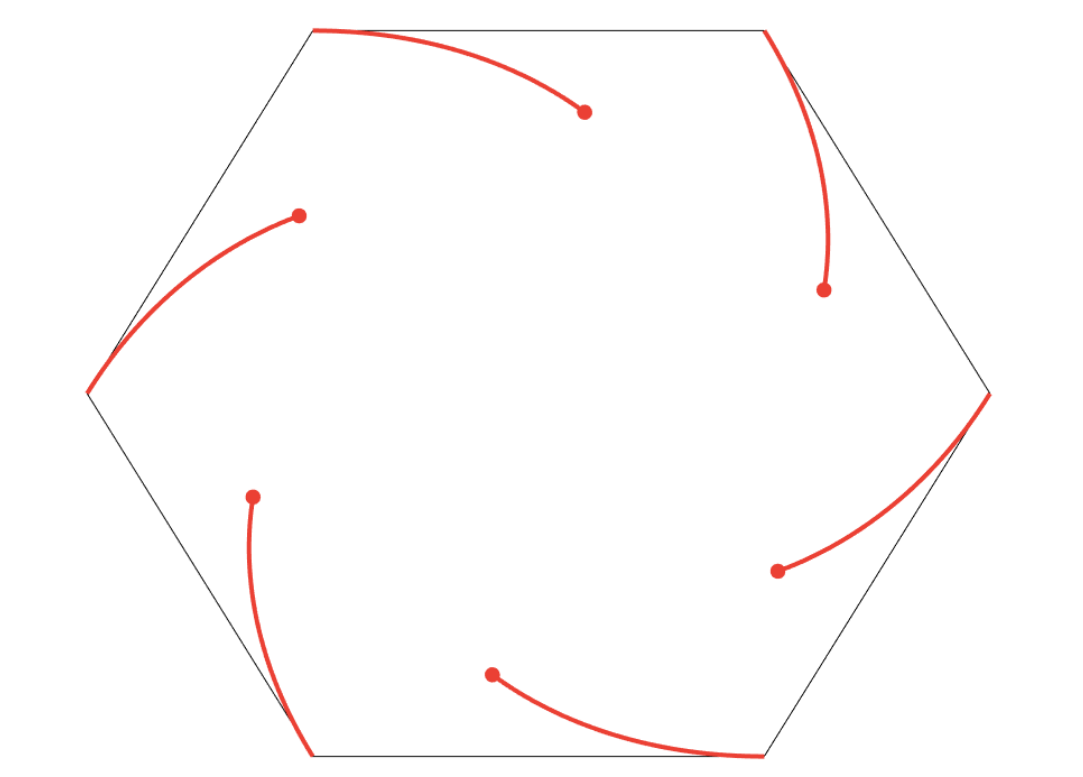
\includegraphics[width=3in]{hexagon1.png}
\end{center}

How long is each snail’s slimy trail?


\section*{Solution:}

This is a pursuit problem, which have been extensively solved by people much smarter than me.
In general, I don't know enough to solve them outright, but I am familiar with the ``easy'' version, which is four pursuers in a square formation.
For this problem, I will call the pursuer A and the target B for any pair of pursuer and target.
The solution to the square problem is that A moves exactly one side length.
Although B is constantly moving, its velocity is perpindicular to the A's velocity, so the distance between A and B only changes based on A's velocity.

Now for the hexagonal version.
I have added labeled the hexagon below, which shows that the exterior angle of each side is 60\textdegree.
This is a basic result of the geometry of a regular hexagon.
This also means that B is moving at \ang{60} relative to A, not perpendicular as in the square case.
Now, B is moving away from A, but at a smaller velocity.
The rate at which it moves away from A is just $\cos(\ang{60})=0.5$.
Now A's relative velocity is only half, so it takes twice as long to reach B.
In this time, it will move twice a single side length, so the solution is
\fcolorbox{red}{white}{\bf 20~m}\,.

\begin{center}
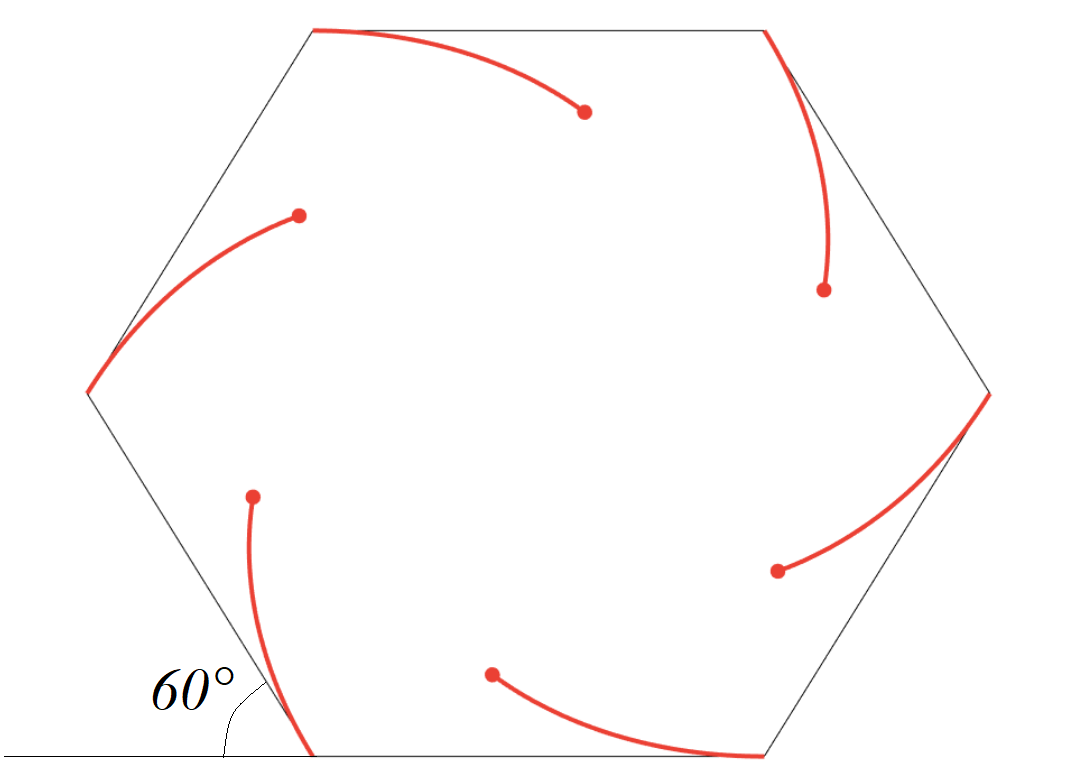
\includegraphics[width=3in]{hexagon2.png}
\end{center}


\end{document}